% Renato Bellotti, October 2018

\documentclass{beamer}

%\usetheme{metropolis}

\usepackage{xcolor}
\usepackage{tikz}
\usetikzlibrary{decorations.pathreplacing}
\usepackage{amsmath}
\usepackage{booktabs}

\setbeamertemplate{navigation symbols}{}

%\newcommand{\UP}{1}
%\newcommand{\RIGHT}{2}
%\newcommand{\DOWN}{3}
%\newcommand{\LEFT}{4}

% (x, y) denotes the top left position of the arrow
% length, x, y, orientation
%\newcommand{\spin}[4][0.5]{
%    \ifthenelse{#4 = \UP}{
%        \draw[->] (#2, #3) -- (#2, #3 + #1);
%    }{}
%    \ifthenelse{#4 = \RIGHT}{
%        \draw[->] (#2, #3) -- (#2 + #1, #3);
%    }{}
%    
%    \ifthenelse{#4 = \DOWN}{
%        \draw[->] (#2, #3) -- (#2, #3);
%    }{}
%}
\newcommand{\up}[0]{$\uparrow$}
\newcommand{\down}[0]{$\downarrow$}

\newenvironment{mybox}{\begin{tcolorbox}[sharp corners=all, frame empty]}{\end{tcolorbox}}


\begin{document}

\begin{frame}{Multi-GPU accelerated multi-spin Monte Carlo simulations of the 2D Ising model}
\begin{tabular}{c c c}
    %\begin{tikzpicture}
%\spin{1}{1}{2}
%\end{tikzpicture}
%\documentclass{article}

%\usepackage{fancyhdr}

%\pagestyle{fancy}
%\fancyfoot{}

%%\newcommand{\UP}{1}
%\newcommand{\RIGHT}{2}
%\newcommand{\DOWN}{3}
%\newcommand{\LEFT}{4}

% (x, y) denotes the top left position of the arrow
% length, x, y, orientation
%\newcommand{\spin}[4][0.5]{
%    \ifthenelse{#4 = \UP}{
%        \draw[->] (#2, #3) -- (#2, #3 + #1);
%    }{}
%    \ifthenelse{#4 = \RIGHT}{
%        \draw[->] (#2, #3) -- (#2 + #1, #3);
%    }{}
%    
%    \ifthenelse{#4 = \DOWN}{
%        \draw[->] (#2, #3) -- (#2, #3);
%    }{}
%}
\newcommand{\up}[0]{$\uparrow$}
\newcommand{\down}[0]{$\downarrow$}

\newenvironment{mybox}{\begin{tcolorbox}[sharp corners=all, frame empty]}{\end{tcolorbox}}


%\begin{document}
{
\setlength{\tabcolsep}{8pt}
\renewcommand{\arraystretch}{1.2}

\begin{tabular}[b]{c c c c c}
    \up & \down & \down & \up & \down \\
    \down & \up & \down & \down & \down \\
    \up & \up & \down & \up & \down \\
    \up & \down & \up & \up & \down
    %$\uparrow$ & $\uparrow$ & $\uparrow$ & $\uparrow$ & $\uparrow$
\end{tabular}
}
%\end{document}

    \textbf{\huge{+}} &
    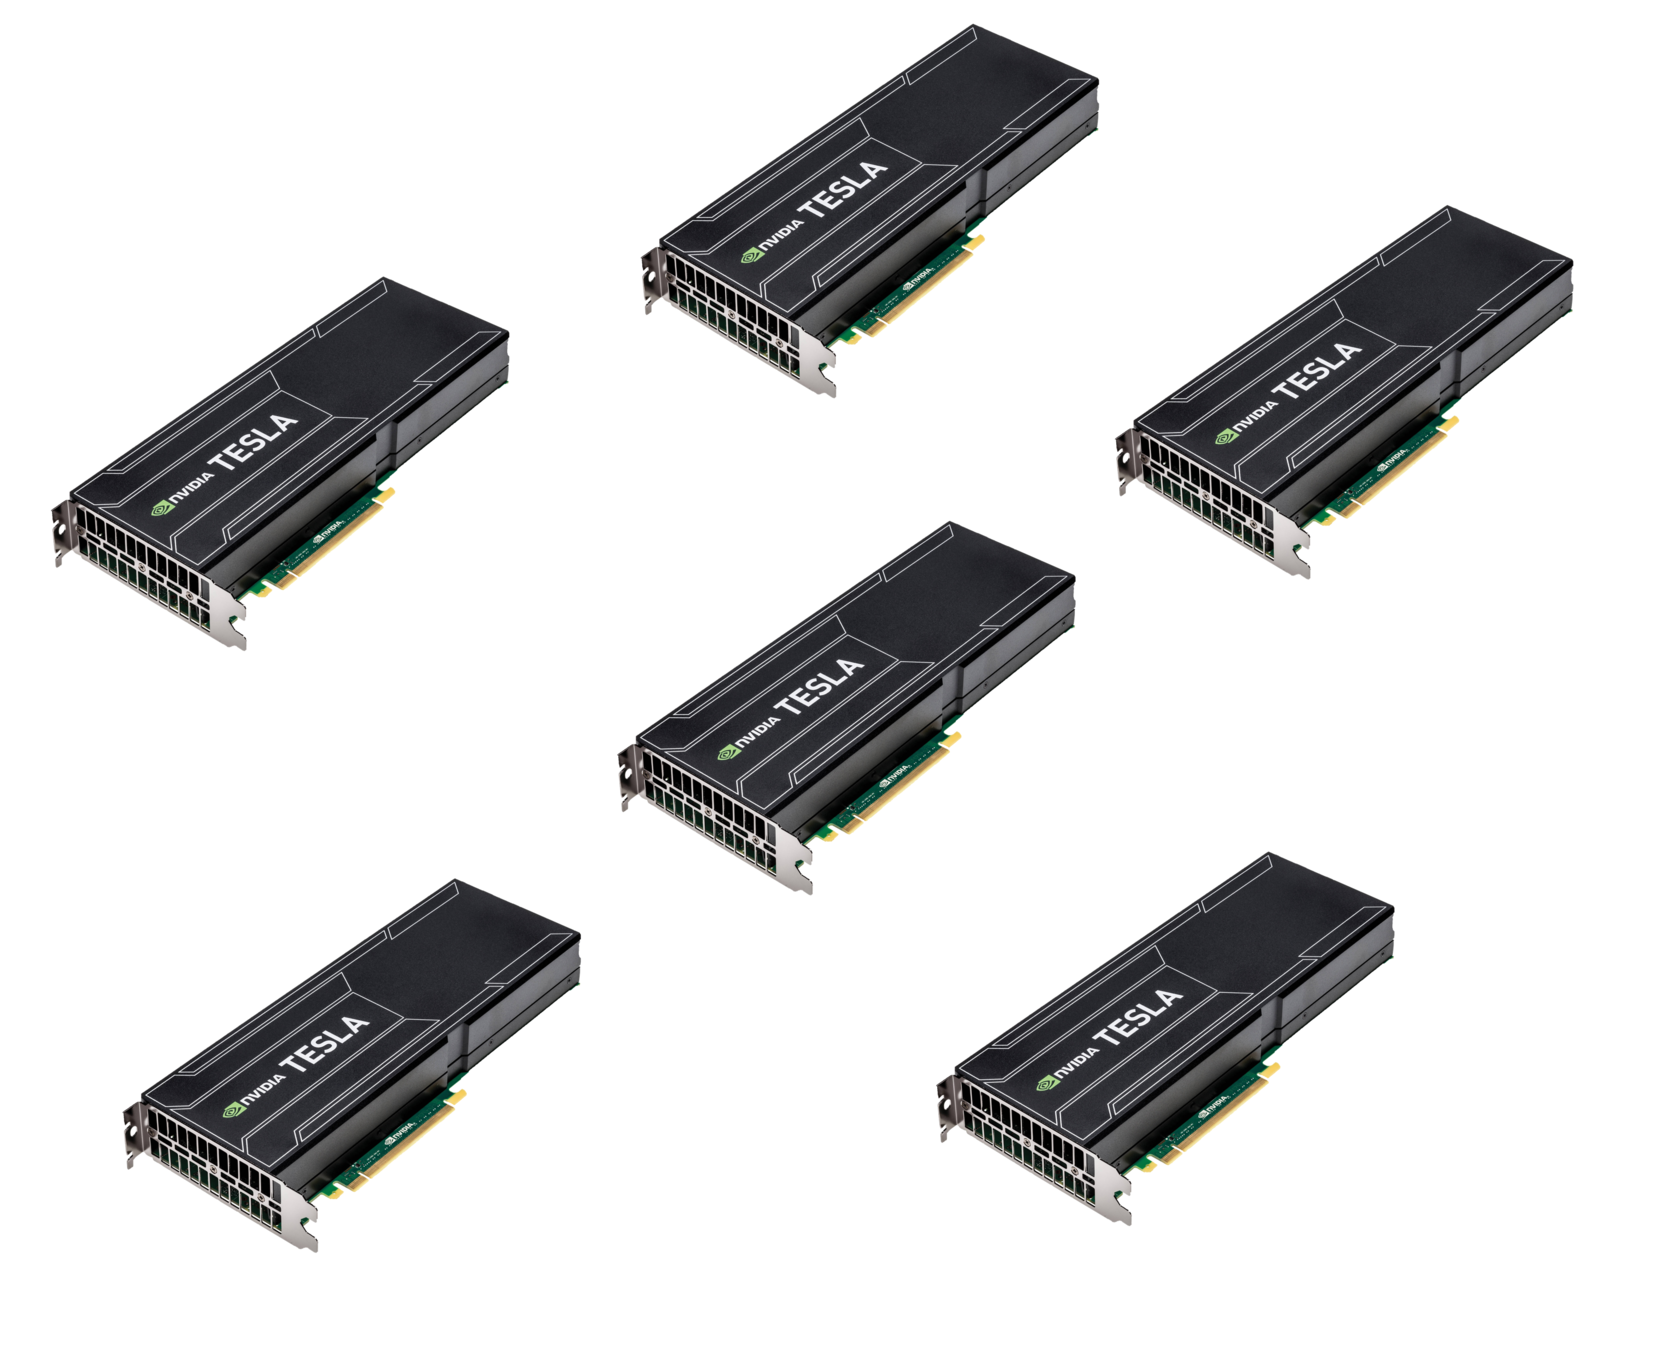
\includegraphics[keepaspectratio=true, width=0.2\paperwidth]{images/multi_gpu.png}
    \textbf{\huge{=}} &
    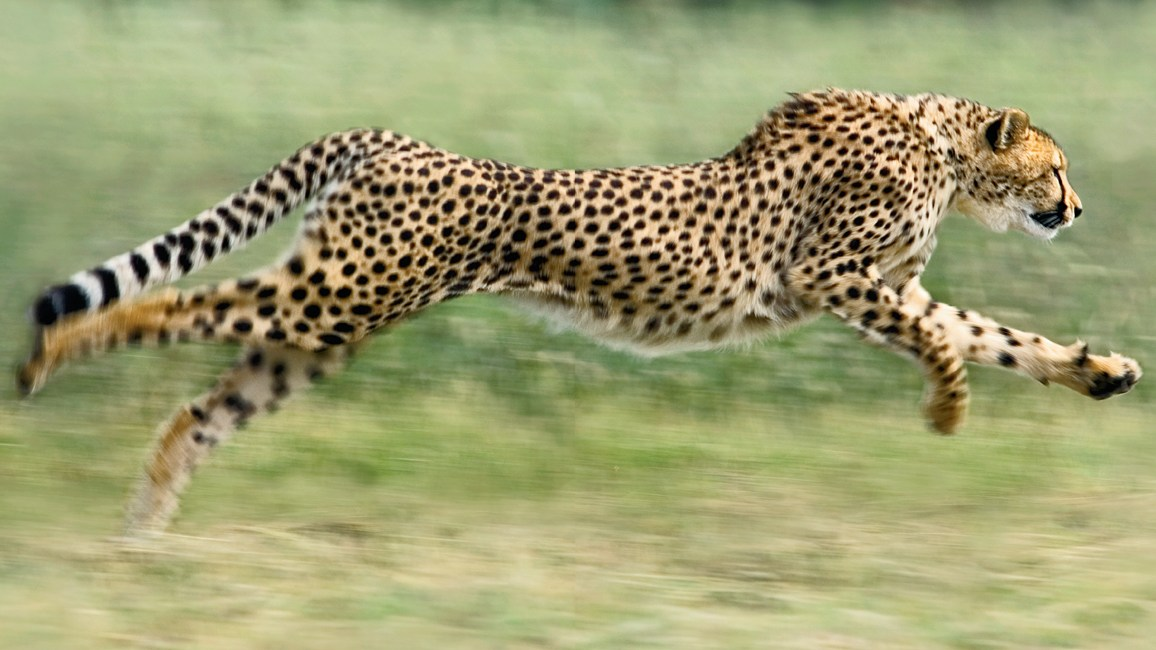
\includegraphics[keepaspectratio=true, width=0.2\paperwidth]{images/cheetah.jpg}
\end{tabular}
\end{frame}

\setcounter{framenumber}{0}
\setbeamertemplate{navigation symbols}{\insertframenumber}

\begin{frame}{What was done?}
    \begin{itemize}
        \item \textbf{Ising model}
            \noindent \ising
        \item \textbf{Metropolis algorithm:}\\
            Efficient sampling
            \begin{equation*}
                p_a = e^{-\frac{E}{k_B T}}
            \end{equation*}
    \end{itemize} \pause
    \vspace{5mm}
    \begin{minipage}{0.2\paperwidth}
        Single core CPU\\
        
\includegraphics[keepaspectratio=true, height=2cm]{images/intel_xeon.jpg}
    \end{minipage} \pause
    \hfill
    \begin{minipage}{0.2\paperwidth}
        Single GPU\\
        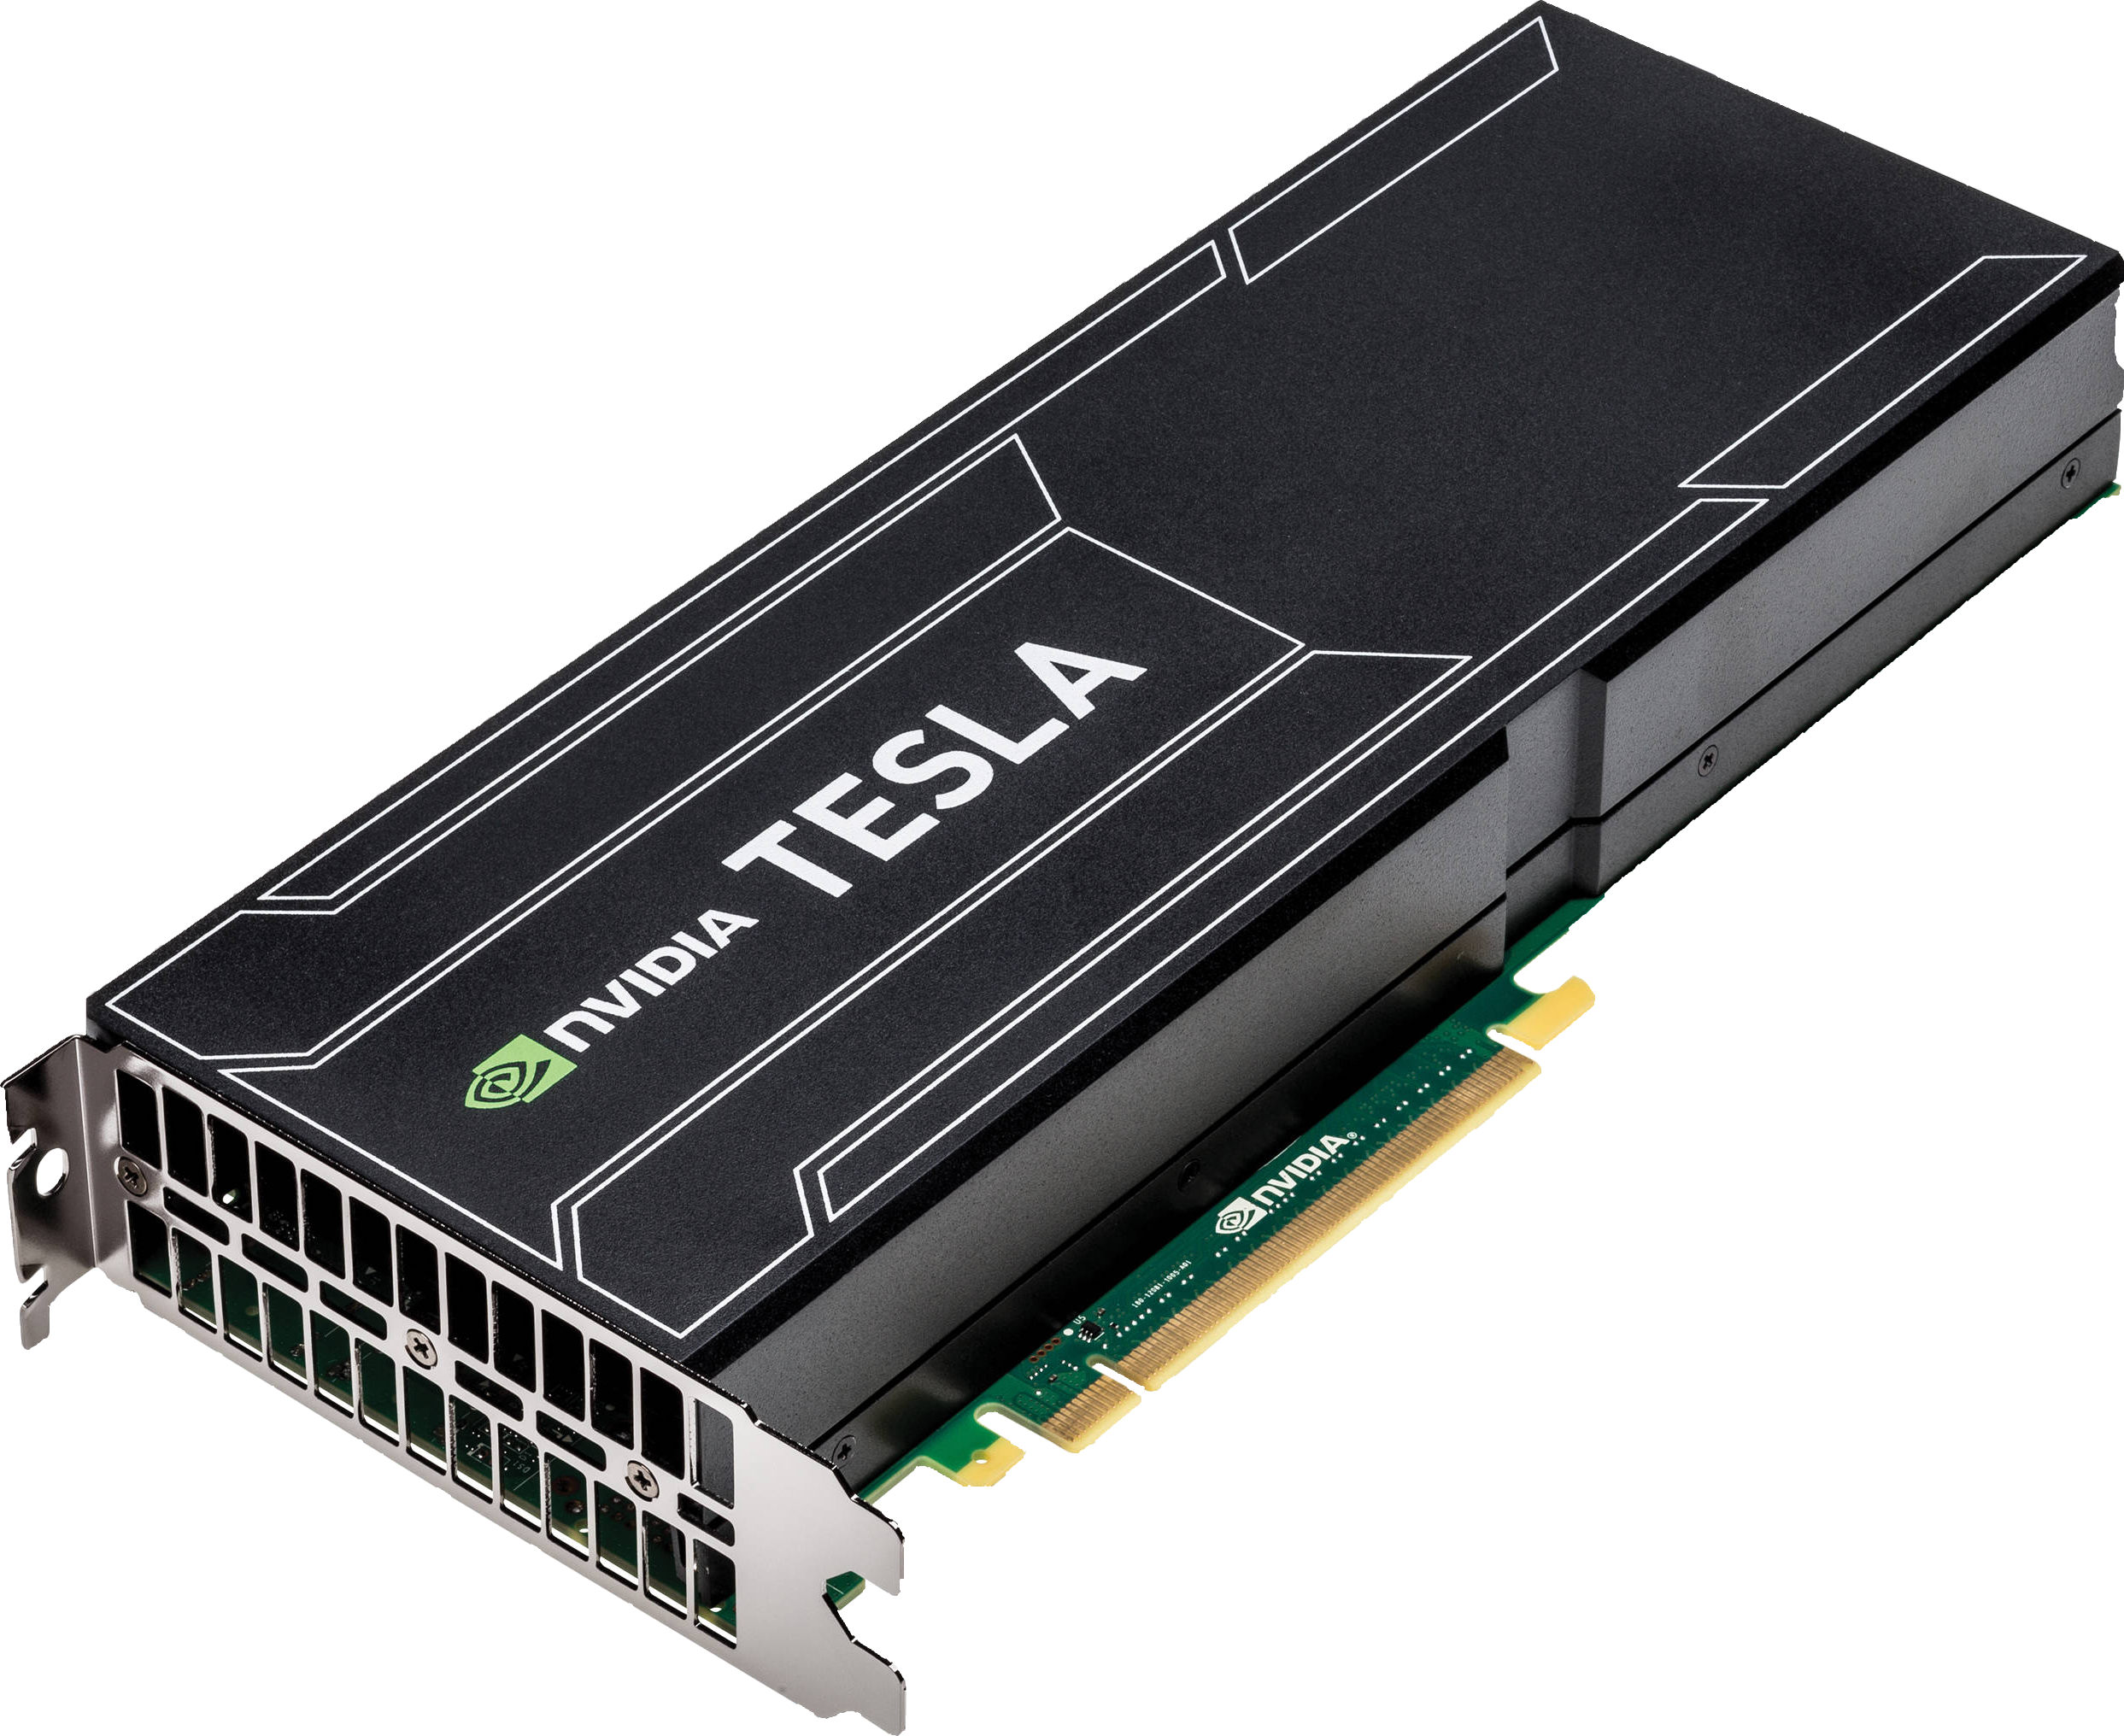
\includegraphics[keepaspectratio=true, height=2cm]{images/gpu_modified.png}
    \end{minipage} \pause
    \hfill
    \begin{minipage}{0.3\paperwidth}
        Mutliple GPUs\\
        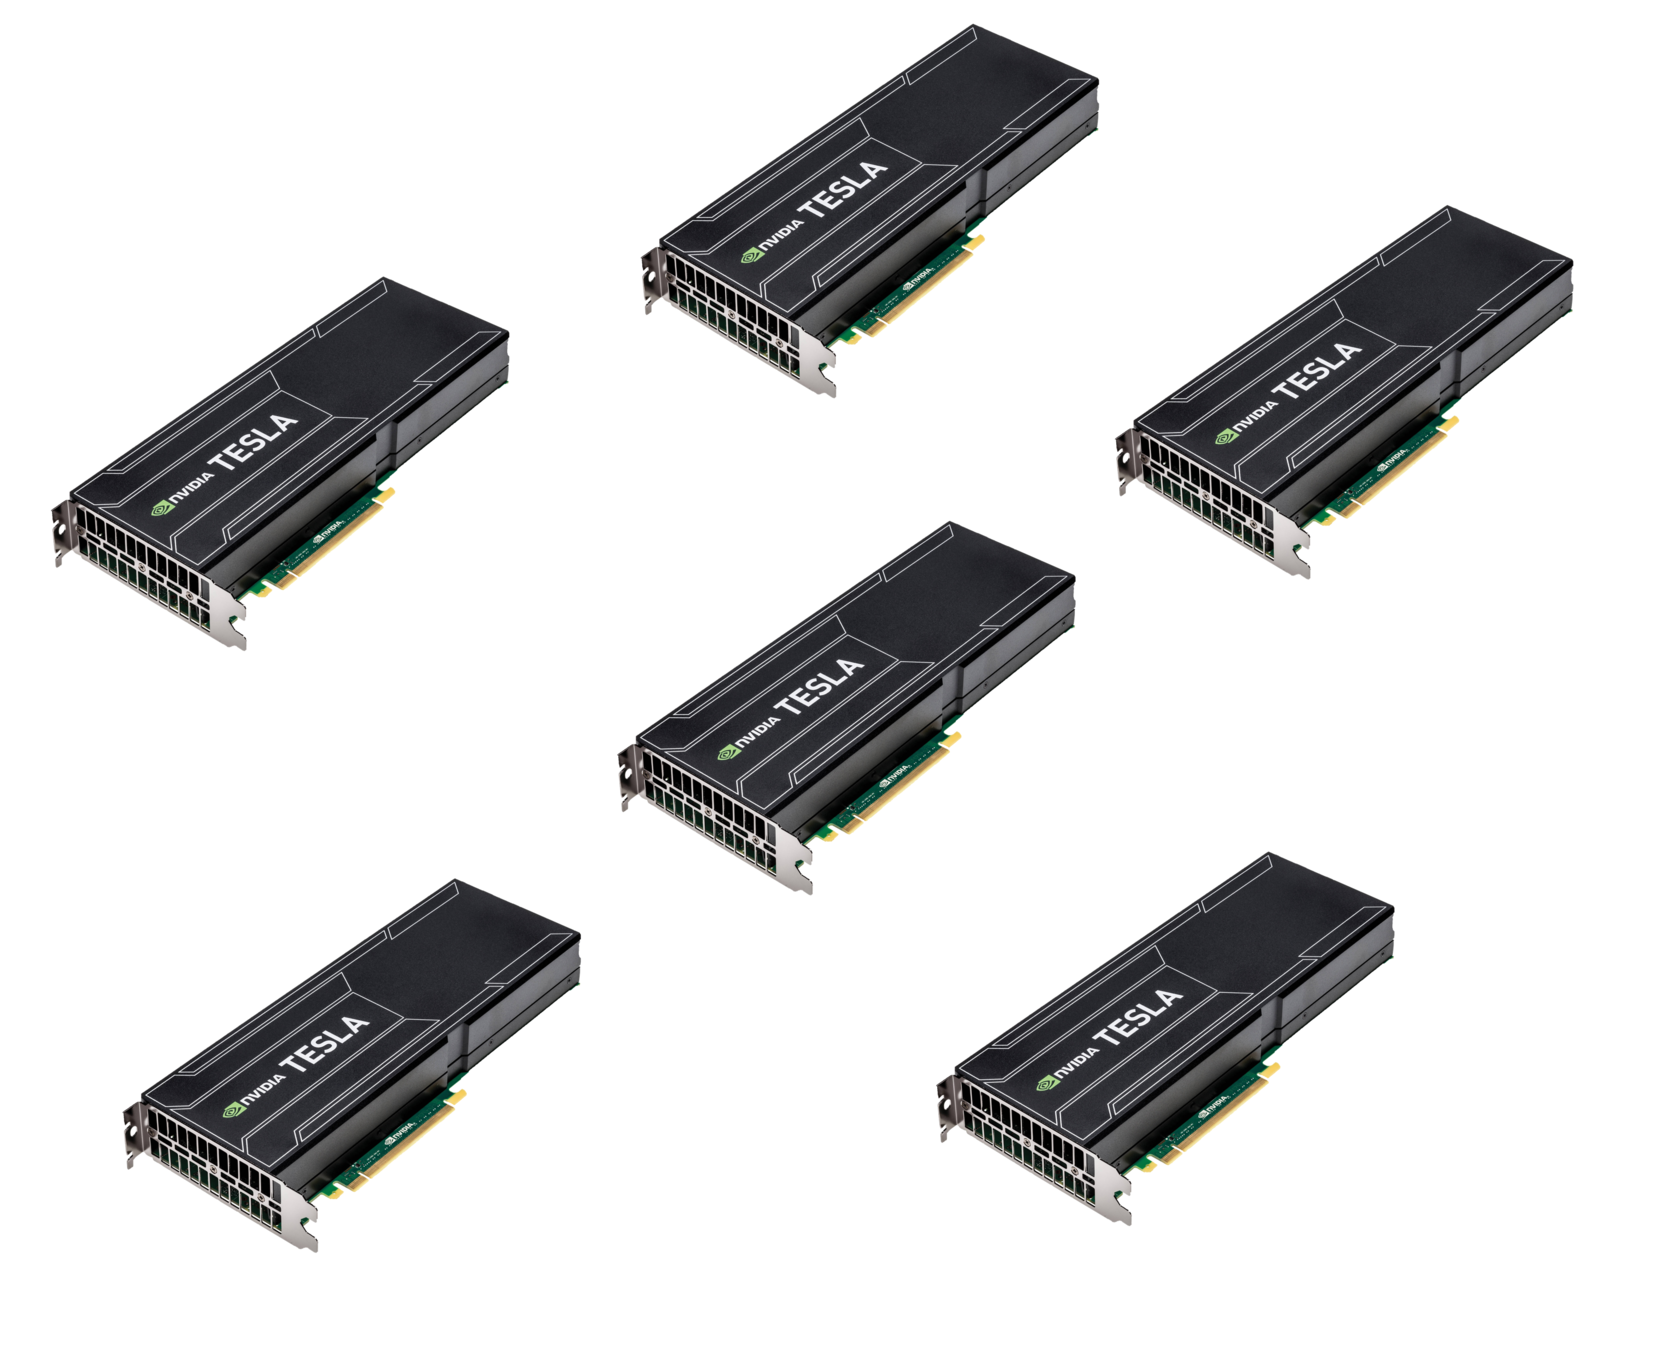
\includegraphics[keepaspectratio=true, height=2cm]{images/multi_gpu.png}
    \end{minipage} \pause
\begin{exampleblock}{}
    How does it scale? Is it worth the effort?
\end{exampleblock}
\end{frame}

\begin{frame}{Ising model I}
\begin{itemize}
    \item Formula:
        \ising \pause
    \item A standard model of statistical physics \pause
    \item classical model \pause
    \item Describes magnets:\\
        \begin{minipage}{0.3\paperwidth}%\begin{tikzpicture}
%\spin{1}{1}{2}
%\end{tikzpicture}
%\documentclass{article}

%\usepackage{fancyhdr}

%\pagestyle{fancy}
%\fancyfoot{}

%%\newcommand{\UP}{1}
%\newcommand{\RIGHT}{2}
%\newcommand{\DOWN}{3}
%\newcommand{\LEFT}{4}

% (x, y) denotes the top left position of the arrow
% length, x, y, orientation
%\newcommand{\spin}[4][0.5]{
%    \ifthenelse{#4 = \UP}{
%        \draw[->] (#2, #3) -- (#2, #3 + #1);
%    }{}
%    \ifthenelse{#4 = \RIGHT}{
%        \draw[->] (#2, #3) -- (#2 + #1, #3);
%    }{}
%    
%    \ifthenelse{#4 = \DOWN}{
%        \draw[->] (#2, #3) -- (#2, #3);
%    }{}
%}
\newcommand{\up}[0]{$\uparrow$}
\newcommand{\down}[0]{$\downarrow$}

\newenvironment{mybox}{\begin{tcolorbox}[sharp corners=all, frame empty]}{\end{tcolorbox}}


%\begin{document}
{
\setlength{\tabcolsep}{8pt}
\renewcommand{\arraystretch}{1.2}

\begin{tabular}[b]{c c c c c}
    \up & \down & \down & \up & \down \\
    \down & \up & \down & \down & \down \\
    \up & \up & \down & \up & \down \\
    \up & \down & \up & \up & \down
    %$\uparrow$ & $\uparrow$ & $\uparrow$ & $\uparrow$ & $\uparrow$
\end{tabular}
}
%\end{document}
\end{minipage}
        \begin{minipage}[c]{0.2\paperwidth} $\mathrel{\widehat{=}}$ \end{minipage}
        \begin{minipage}{0.2\paperwidth}
\includegraphics[keepaspectratio=true, width=0.3\paperwidth]{images/magnet.jpg}\end{minipage} \pause
    \item System sizes: $100'000 \times 100'000$
\end{itemize}
\end{frame}

\begin{frame}{Ising model II}
    Nearest neighbour interactions only!
    \ising \pause
    \vspace{1cm}
    \begin{minipage}{0.3\paperwidth}{
\setlength{\tabcolsep}{8pt}
\renewcommand{\arraystretch}{1.2}

\begin{tabular}[b]{c c c c c}
    \rup & \rup & \rup & \rup & \rdown \\
    \rdown & \rup & \gdown & \rdown & \rup \\
    \rup & \rdown & \rup & \rdown & \rup \\ 
\end{tabular}
}
\end{minipage}
    {\Huge$\Rightarrow$}
    \begin{minipage}{0.2\paperwidth}{
\setlength{\tabcolsep}{8pt}
\renewcommand{\arraystretch}{1.2}

\begin{tabular}[b]{c c c c c}
    \up & \up & \rup & \up & \down \\
    \down & \rup & \gdown & \rdown & \up \\
    \up & \down & \rup & \down & \up \\ 
\end{tabular}
}
\end{minipage} \pause
    
    Calculation of energy: $\mathcal{O}\left( n^2 \right) \Rightarrow \mathcal{O}\left( n \right)$
\end{frame}

\begin{frame}{Metropolis algorithm}
\begin{itemize}
    \item \textbf{Goal:} Sample phase space\\
        \vspace{3mm}
        \begin{minipage}[c]{0.4\textwidth}
            %\begin{tikzpicture}
%\spin{1}{1}{2}
%\end{tikzpicture}
%\documentclass{article}

%\usepackage{fancyhdr}

%\pagestyle{fancy}
%\fancyfoot{}

%%\newcommand{\UP}{1}
%\newcommand{\RIGHT}{2}
%\newcommand{\DOWN}{3}
%\newcommand{\LEFT}{4}

% (x, y) denotes the top left position of the arrow
% length, x, y, orientation
%\newcommand{\spin}[4][0.5]{
%    \ifthenelse{#4 = \UP}{
%        \draw[->] (#2, #3) -- (#2, #3 + #1);
%    }{}
%    \ifthenelse{#4 = \RIGHT}{
%        \draw[->] (#2, #3) -- (#2 + #1, #3);
%    }{}
%    
%    \ifthenelse{#4 = \DOWN}{
%        \draw[->] (#2, #3) -- (#2, #3);
%    }{}
%}
\newcommand{\up}[0]{$\uparrow$}
\newcommand{\down}[0]{$\downarrow$}

\newenvironment{mybox}{\begin{tcolorbox}[sharp corners=all, frame empty]}{\end{tcolorbox}}


%\begin{document}
{
\setlength{\tabcolsep}{8pt}
\renewcommand{\arraystretch}{1.2}

\begin{tabular}[b]{c c c c c}
    \up & \down & \down & \up & \down \\
    \down & \up & \down & \down & \down \\
    \up & \up & \down & \up & \down \\
    \up & \down & \up & \up & \down
    %$\uparrow$ & $\uparrow$ & $\uparrow$ & $\uparrow$ & $\uparrow$
\end{tabular}
}
%\end{document}

        \end{minipage}
        \begin{minipage}[c]{0.2\textwidth} {\Huge $\stackrel{!}{\sim}$} \end{minipage}
        \begin{minipage}[c]{0.3\textwidth} {\Huge $e^{-\frac{E}{k_B T}}$} \end{minipage} \pause
    \vspace{2mm}
    \item \textbf{Algorithm:}\\ \pause
            1.) Propose new state: Random spin flips!\\
            \vspace{2mm}
            \begin{minipage}{0.3\textwidth}
                {
\setlength{\tabcolsep}{8pt}
\renewcommand{\arraystretch}{1.2}

\begin{tabular}[b]{c c c c c}
    \up & \down & \down & \up & \up \\
    \down & \up & \rdown & \up & \up \\
    \up & \up & \up & \down & \down \\
\end{tabular}
}

            \end{minipage}
            \hfill
            \begin{minipage}[c]{0.2\textwidth} {\Huge $\Rightarrow$} \end{minipage}
            \begin{minipage}[c]{0.3\textwidth}
                {
\setlength{\tabcolsep}{8pt}
\renewcommand{\arraystretch}{1.2}

\begin{tabular}[b]{c c c c c}
    \up & \down & \down & \up & \up \\
    \down & \up & \rup & \up & \up \\
    \up & \up & \up & \down & \down \\
\end{tabular}
}

            \end{minipage}\\ \pause
            2.) Accept the new configuration: $p_a = e^{-\frac{\Delta E}{k_B T}}$
\end{itemize}
\end{frame}

\begin{frame}{Single core CPU: Data structure}
\begin{itemize}
    \item Multi-spin coding: 1~spin $\mathrel{\widehat{=}}$ 1~bit \pause
    \item Group spins in groups of size 32 (int)\\
        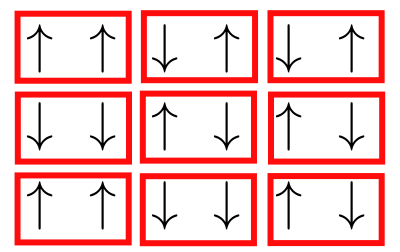
\includegraphics[keepaspectratio=true, width=0.7\textwidth]{images/grouped_spins_modified.png} \pause
    \item 100'000 $\times$ 100'000 lattice: $\approx$~1.2~GB
\end{itemize}
\end{frame}

\begin{frame}{Single core CPU: Algorithm I}
    \begin{minipage}{0.5\textwidth}
        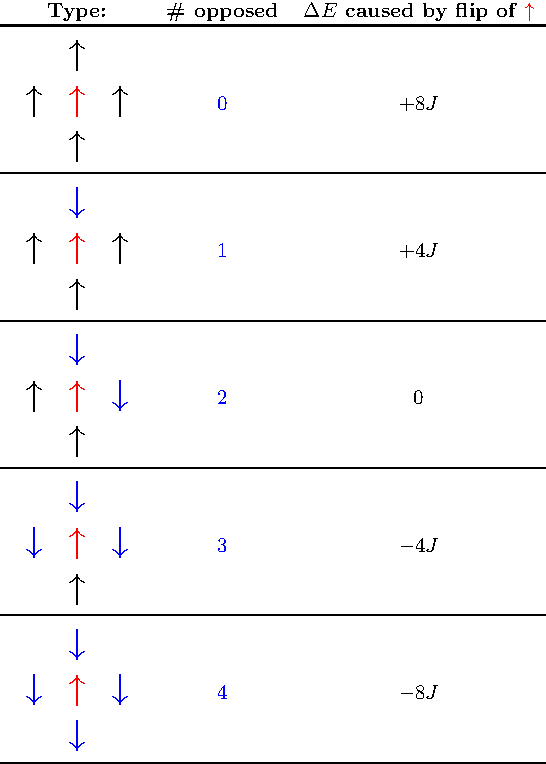
\includegraphics[keepaspectratio=true, scale=0.6]{images/cases.pdf}\\
    \end{minipage} \pause
    \hfill
    \begin{minipage}{0.4\textwidth}
        \begin{equation*}
            p_a = e^{-\frac{\Delta E}{k_B T}}
        \end{equation*} \pause
        \begin{exampleblock}{}
            Count \#opposed spins!
        \end{exampleblock}
    \end{minipage}
    %\begin{tikzpicture}
    %    \draw [decorate,decoration={brace,amplitude=10pt},xshift=+4pt,yshift=20pt] (0.5,12.5) -- (0.5,7.0) node [black,midway,xshift=+0.7cm] {\footnotesize $P_1$};
    %\end{tikzpicture}
\end{frame}

\begin{frame}{Single core CPU: Algorithm II}
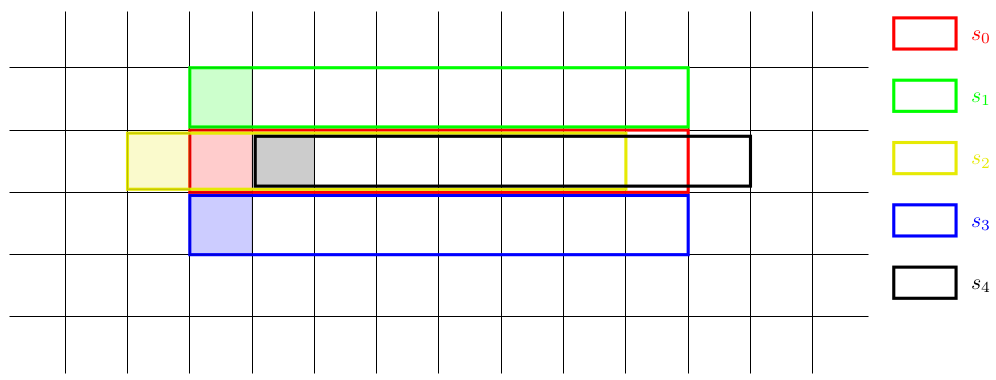
\includegraphics[keepaspectratio=true, width=\textwidth]{images/single_core2.png}\\ \pause
\begin{minipage}{0.5\textwidth}
    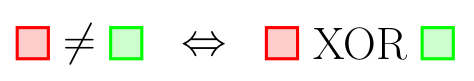
\includegraphics[keepaspectratio=true, width=\textwidth]{images/single_core3.png}\\ \pause
    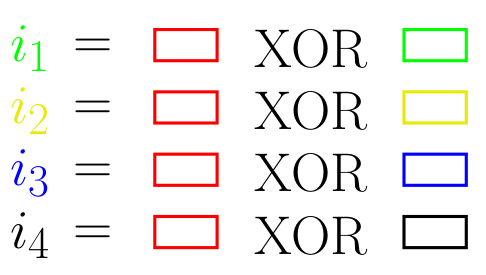
\includegraphics[keepaspectratio=true, width=\textwidth]{images/single_core4.png} \pause
\end{minipage}
\hfill\vline\hfill
%\hfill
\begin{minipage}{0.4\textwidth}
    Combine with acceptance probability:
    \begin{equation*}
        i_1 + i_2 + i_3 + i_4 + 2 \text{exp}_8 + \text{exp}_4 \geq 2
    \end{equation*}
\end{minipage}
\end{frame}

\end{document}
